% ======================================================================
\subsection{Modelo conceptual}
El presente documento representa un análisis de los datos que construyen
el sistema OMI y cómo estos se relacionan. El documento describe el 
modelo conceptual de datos del sistema mediante diagramas de clases. Las 
clases son organizadas en paquetes para facilitar la modularidad del sistema
y su entendimiento. 

El proceso de interpretar conciste en tomar codigo fuente, procesarlo y ejecutar 
su significado semántico. Por tanto el modelo de datos estará constituido por
entidades que guardan un significado concreto y preciso dentro del lenguaje.
Estos elementos, que representan la unidad semántica mínima, 
son denominados nodos ejecutables, debido a que cuando 
son ejecutados producen el resultado semántico asociado.  Muchos nodos ejecutables
por si solos no presentan un resultado semántico completo, por lo que precisan de otros
nodos. 

El diagrama general de paquetes describe los paquetes que componen el 
sistema según el carácter funcional de las entidades que contienen. Un 
paquete podrá contener clases u otros paquetes.

El paquete ``interpreter'' describe las entidades que procesan  
el contenido fuente según el léxico y la gramática del lenguaje OMI. 
El objetivo es generar el árbol de nodos ejecutables correspondiente al
programa. Al procesarse este árbol se aplicará la semántica que encierran 
las líneas de código del contenido fuente, produciéndose de esta forma la ejecución del programa.

El paquete ``runNode'' describe el nodo ejecutable y aquellos tipos de nodos derivados
de este, que son abstractos y que serán extendidos por tipos más específicos.

El paquete ``typeData'' describe los nodos correspondientes a los tipos de datos básicos 
que pueden ser manipulados por el sistema. 

El paquete ``error'' describe el sistema de errores y los nodos ejecutables que permiten
su control.

El paquete ``extensions'' describe el sistema de extensiones del interprete, el cual
permite extender la funcionalidades del lenguaje de una forma dinámica. Además contiene dos
el modelado de dos extensiones concretas.  

Los paquetes siguientes categorizan y agrupan nodos ejecutables según la funcionalidad 
que encierran y el tipo de dato sobre el que operan. 

El último paquete ``rtree'' describe el modelo de datos correspondiente al sistema 
software cliente. Una aplicación web que hace uso del interprete de forma online
y representa el estado de este.

\begin{center}
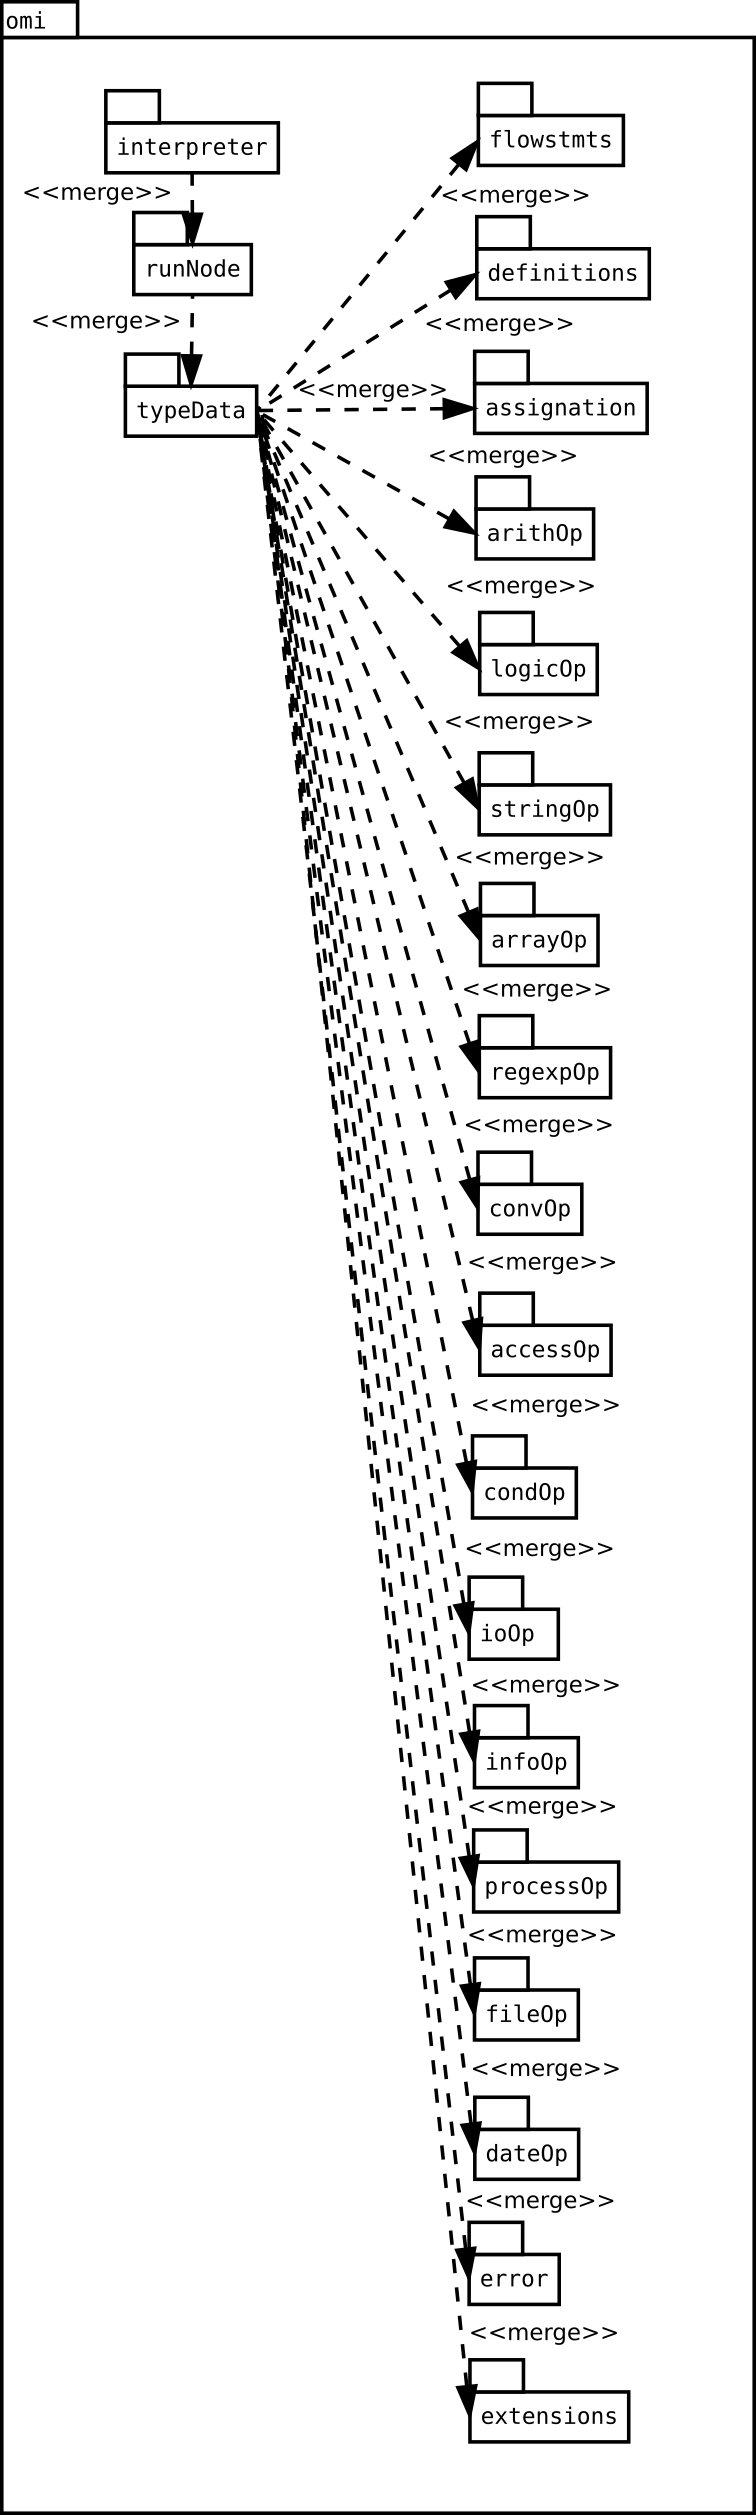
\includegraphics[scale=0.3]{package-omi.png} \\
\end{center}
% ======================================================================
\pagebreak
\subsubsection{Intérprete}
El sistema OMI se corresponde con un interprete que opera sobre 
un contenido fuente escrito en el lenguaje con el mismo nombre. 
El interprete se compone de un analizador sintáctico que encierra la 
gramática del lenguaje, esta es descrita a partir de una serie de tokens.

El analizador sintáctico se vale de un analizador léxico que validará 
y obtendrá los tokens (bajo petición) desde el código fuente.
El analizador léxico debe controlar el fichero que contiene el código fuente, 
así como la línea y posición que se encuentra procesando en el mismo.

Los tokens obtenidos se definen por un identificador y la línea del código fuente en la que se generó,
además pueden tener asociado un valor que puede ser numérico o cadena. Serán utilizados 
por el analizador sintáctico para determinar las reglas gramaticales que se deben aplicar y
construir el árbol sintáctico correspondiente. Este árbol está formado 
por nodos denominados ejecutables, dado que al ser procesados en profundidad se llevará 
a cabo la ejecución del programa. Los nodos ejecutables dan singnificado semántico a 
cada una de las sentencias que componen el contenido fuente.

El interprete se compone además de un contexto denominado principal, que será sobre el que 
opere de forma predeterminada. Un contexto está formado por una serie de tablas de símbolos 
que serán manipuladas por ciertos nodos ejecutables cuando sean procesados. Estas tablas guardan 
referencias a nodos ejecutables correspondientes a símbolos variables, funciones y clases de objetos 
que son definidos en el código fuente. Existen determinados nodos que al ser ejecutados pueden 
cambiar el contexto en uso.

El interprete es ejecutado con una serie de argumentos que alteran su funcionamiento.

\begin{center}
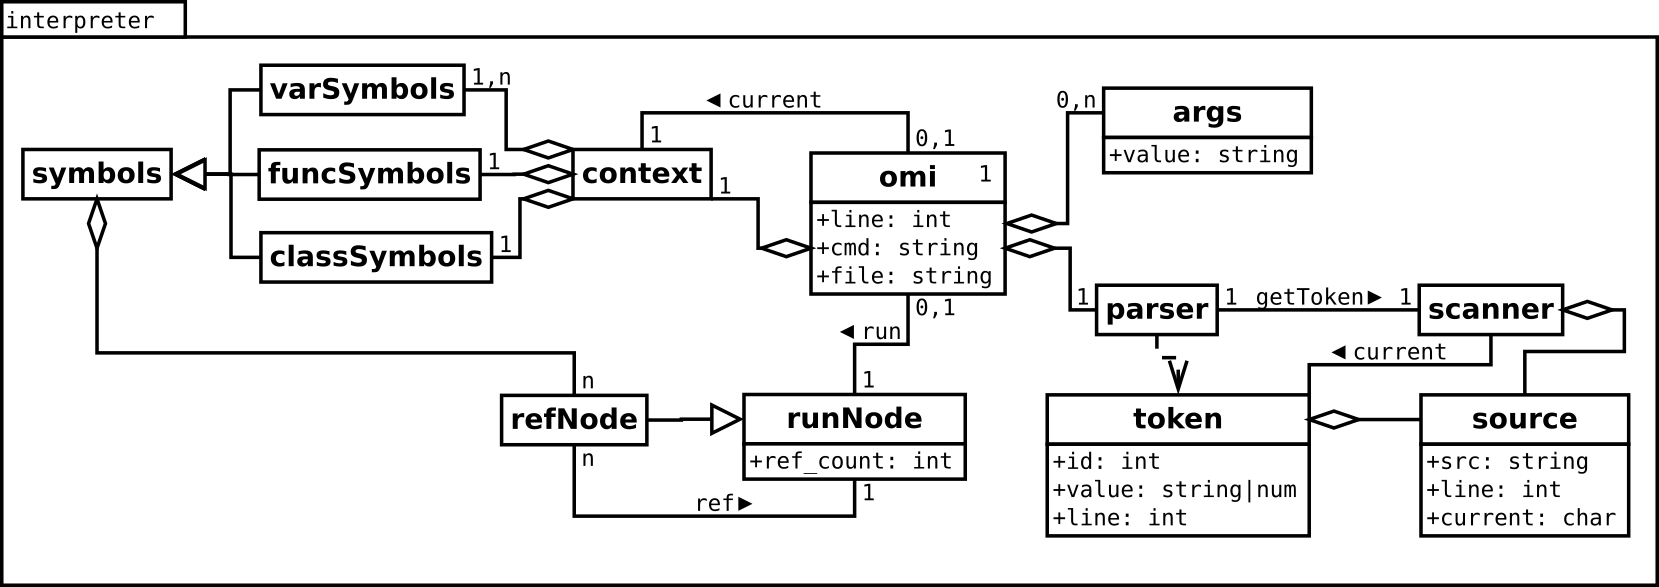
\includegraphics[scale=0.3]{interpreter.png} \\
\end{center}
% ----------------------------------------------------------------------
\pagebreak
\subsubsection{Nodos ejecutables}
Se definen un nodo ejecutable para cada aspecto o funcionalidad que contemple el lenguaje.
Cada sentencia se corresponde con un nodo ejecutable, que a su vez puede estar compuestos de otros
nodos. Cada nodo ejecutable guarda el número de nodos que lo referencian para que se pueda hacer un uso 
óptimo del mismo.

Las expresiones son nodos ejecutables que tomarán un valor tras ser procesados. Generalmente forman parte de otros 
nodos correspondientes a sentencias u otras expresiones. El valor que toman pueden ser de un tipo determinado y conocido (numérico, lógico, etc), 
o de tipo indeterminado o no conocido hasta que el nodo es procesado. 

Las expresiones de tipo determinado son extendidas por cada tipo de dato soportado por el lenguaje. Además 
pueden ser consideradas tipos de objetos y estar así asociadas a una clase. De esta forma toda expresión puede disponer
de métodos y atributos según el tipo de dato que guarde.

Las expresiones de tipo indeterminado se componen de una referencia al nodo que guarda el valor tras la ejecución, este podrá ser una 
expresión de tipo determinado.

Las expresiones son nodos imprimibles lo que significa que tienen una representación gráfica asociada que puede ser volcada en la
salida estándar.

\begin{center}
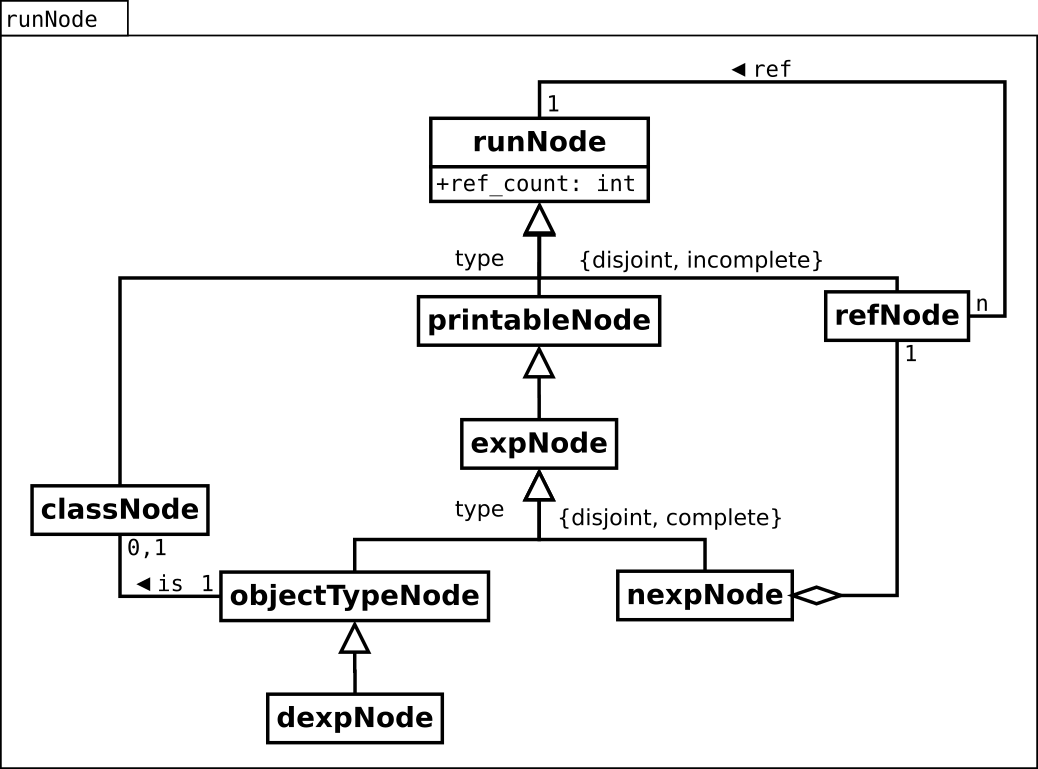
\includegraphics[scale=0.4]{runNode.png} \\
\end{center}
% ----------------------------------------------------------------------
\pagebreak
\subsubsection{Tipos de datos}
Este paquete contiene los nodos que representan expresiones con tipos de datos definidos.
Se describe cada tipo de dato como un nodo con un valor asociado (en algunos casos el tipo puede comprender un único valor).

Muchos nodos son especializaciones de tipos de datos, correspondiéndose con expresiones que 
guardan un valor del tipo de dato al que extienden. Así por ejemplo los nodos de operaciones aritméticas
generalmente extenderán al nodo del mismo tipo de dato. 

Algunos nodos de tipos datos son concretados por nodos que representan un valor constante de dicho tipo de dato.
 
\begin{center}
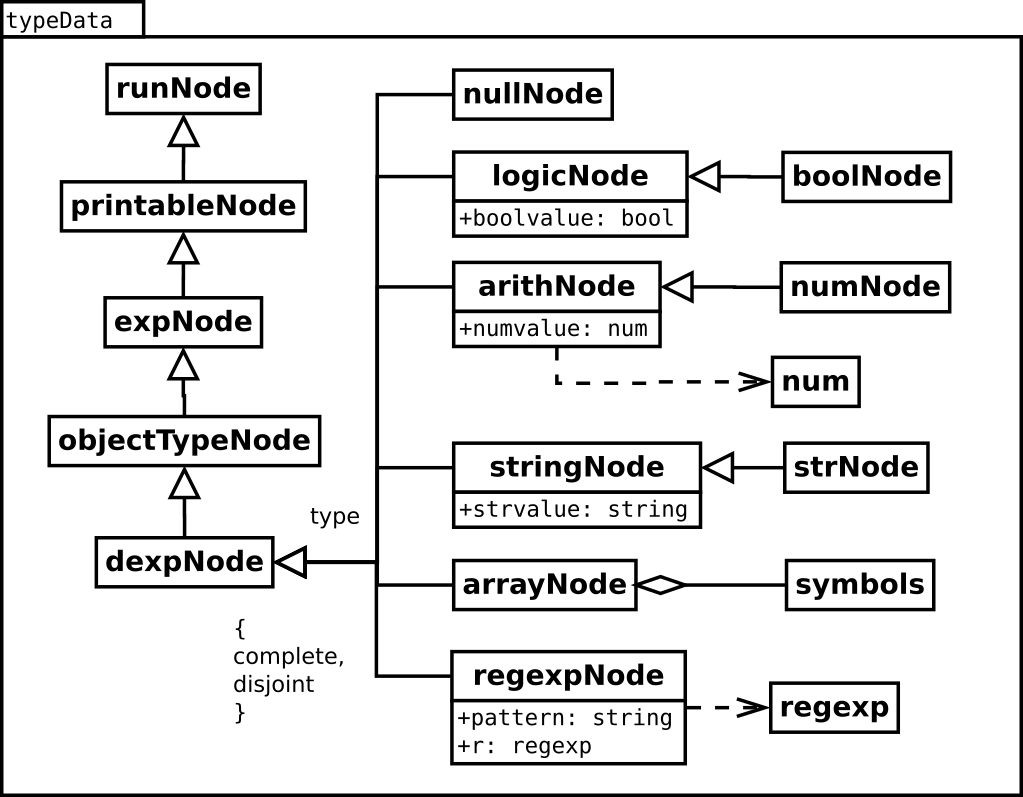
\includegraphics[scale=0.4]{typeData.png} \\
\end{center}
% ----------------------------------------------------------------------
\pagebreak
\subsubsection{Sentencias de control de flujo}
\begin{center}
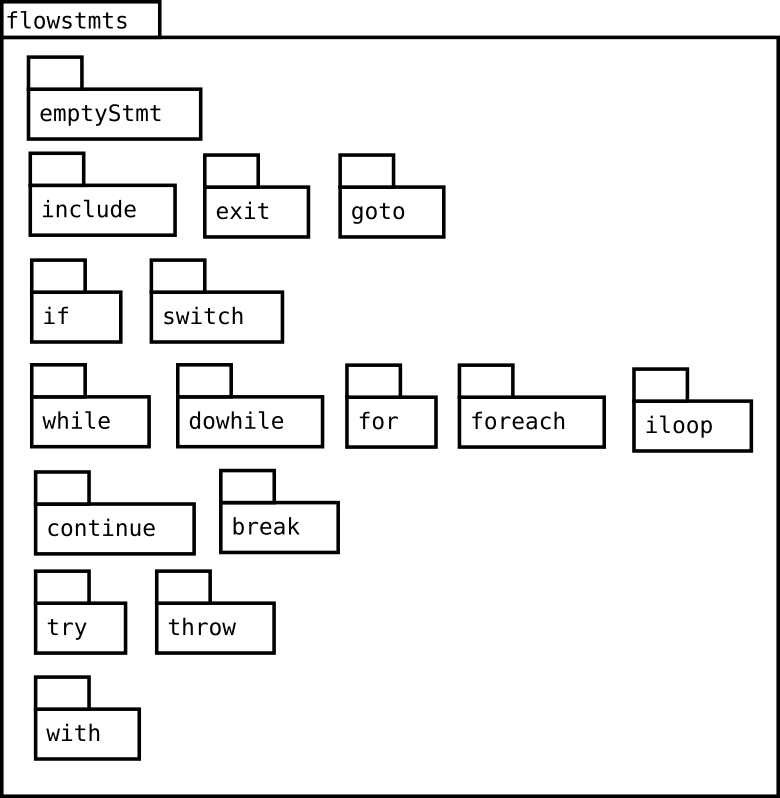
\includegraphics[scale=0.4]{flowstmts.png} \\
\end{center}

\paragraph{Sentencia}
\begin{center}
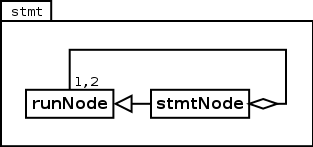
\includegraphics[scale=0.4]{stmt.png} \\
\end{center}

\paragraph{Sentencia vacía}
\begin{center}
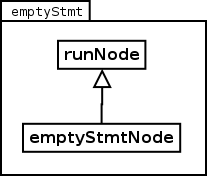
\includegraphics[scale=0.4]{emptyStmt.png} \\
\end{center}

\paragraph{include}
\begin{center}
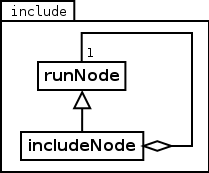
\includegraphics[scale=0.4]{include.png} \\
\end{center}

\paragraph{exit}
\begin{center}
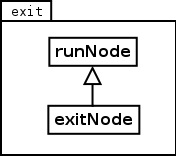
\includegraphics[scale=0.4]{exit.png} \\
\end{center}

\paragraph{goto}
\begin{center}
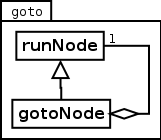
\includegraphics[scale=0.4]{goto.png} \\
\end{center}

\paragraph{if}
\begin{center}
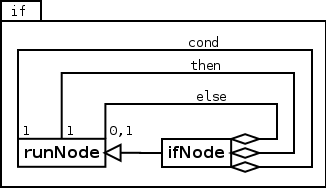
\includegraphics[scale=0.4]{if.png} \\
\end{center}

\paragraph{switch}
\begin{center}
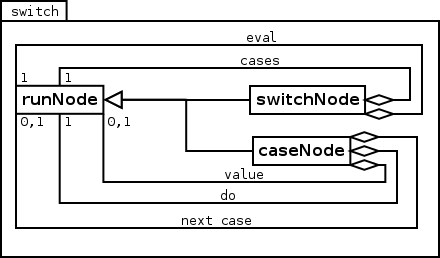
\includegraphics[scale=0.4]{switch.png} \\
\end{center}

\paragraph{while}
\begin{center}
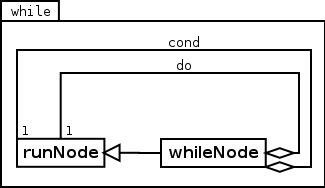
\includegraphics[scale=0.4]{while.png} \\
\end{center}


\paragraph{do...while}
\begin{center}
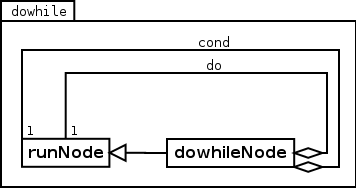
\includegraphics[scale=0.4]{dowhile.png} \\
\end{center}

\paragraph{for}
\begin{center}
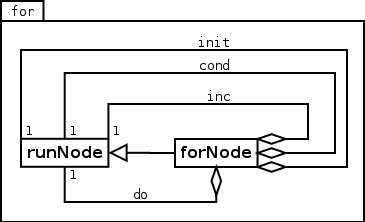
\includegraphics[scale=0.4]{for.png} \\
\end{center}

\paragraph{foreach}
\begin{center}
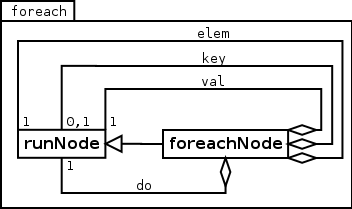
\includegraphics[scale=0.4]{foreach.png} \\
\end{center}

\paragraph{iloop}
\begin{center}
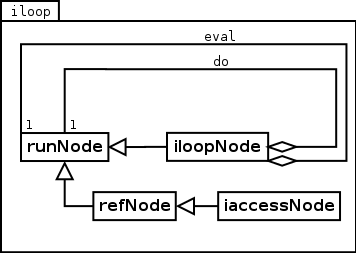
\includegraphics[scale=0.4]{iloop.png} \\
\end{center}


\paragraph{continue}
\begin{center}
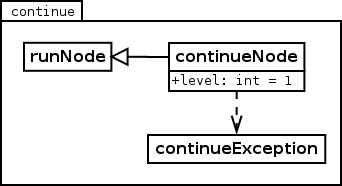
\includegraphics[scale=0.4]{continue.png} \\
\end{center}

\paragraph{break}
\begin{center}
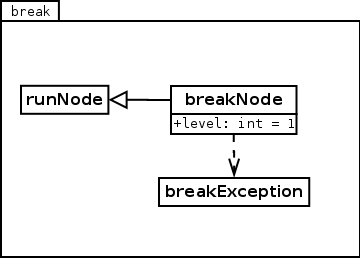
\includegraphics[scale=0.4]{break.png} \\
\end{center}

\paragraph{try}
\begin{center}
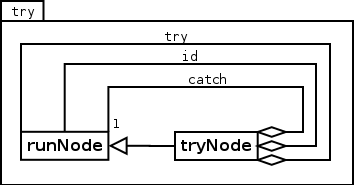
\includegraphics[scale=0.4]{try.png} \\
\end{center}

\paragraph{throw}
\begin{center}
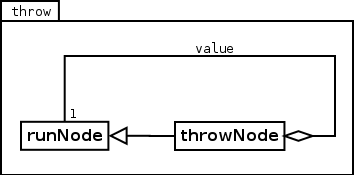
\includegraphics[scale=0.4]{throw.png} \\
\end{center}


\paragraph{with}
\begin{center}
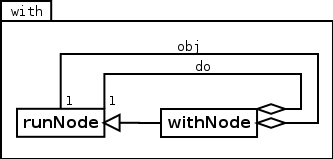
\includegraphics[scale=0.4]{with.png} \\
\end{center}
% ----------------------------------------------------------------------
\pagebreak
\subsubsection {Definiciones}
\begin{center}
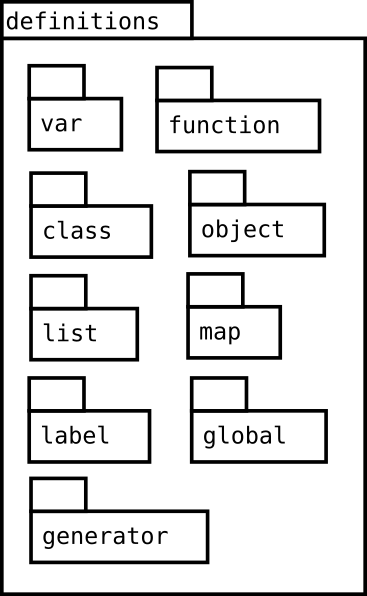
\includegraphics[scale=0.4]{definitions.png} \\
\end{center}

\paragraph {Variables}
\begin{center}
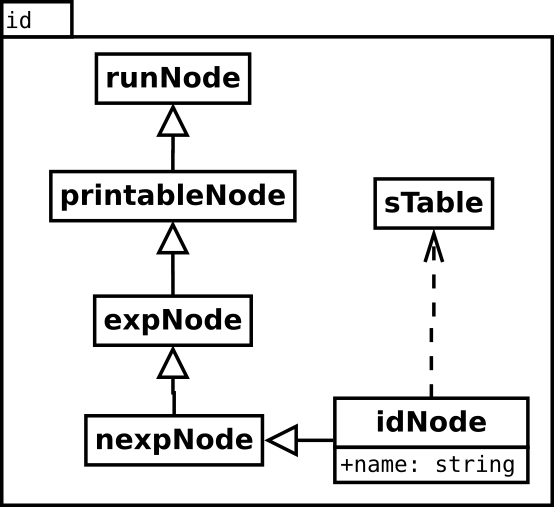
\includegraphics[scale=0.4]{id.png} \\
\end{center}

\paragraph {Funciones}
\begin{center}
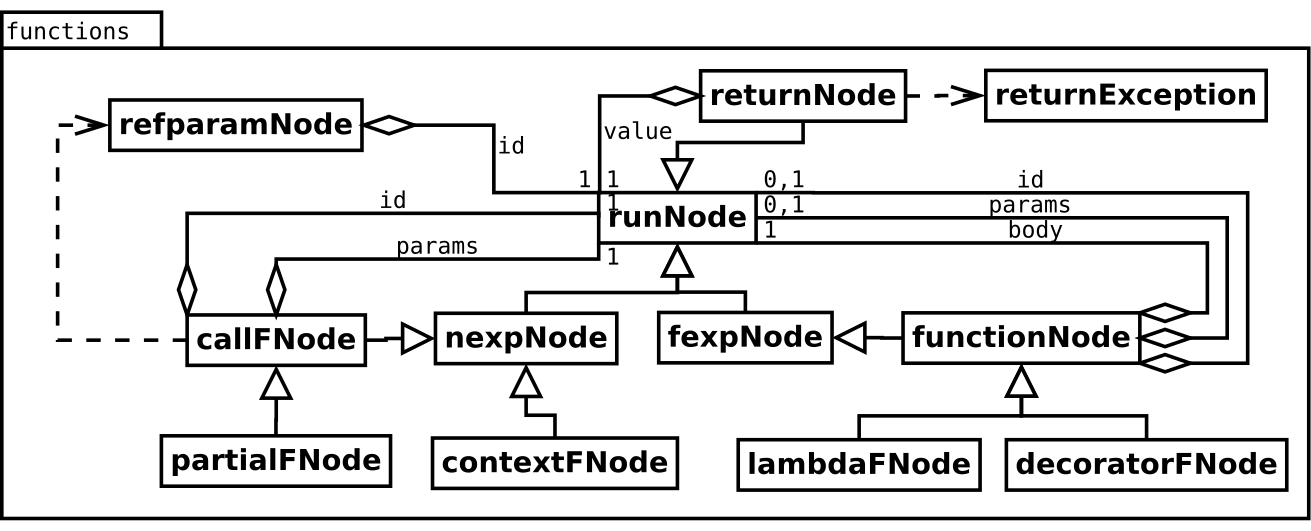
\includegraphics[scale=0.4]{functions.png} \\
\end{center}

\paragraph {Clases}
\begin{center}
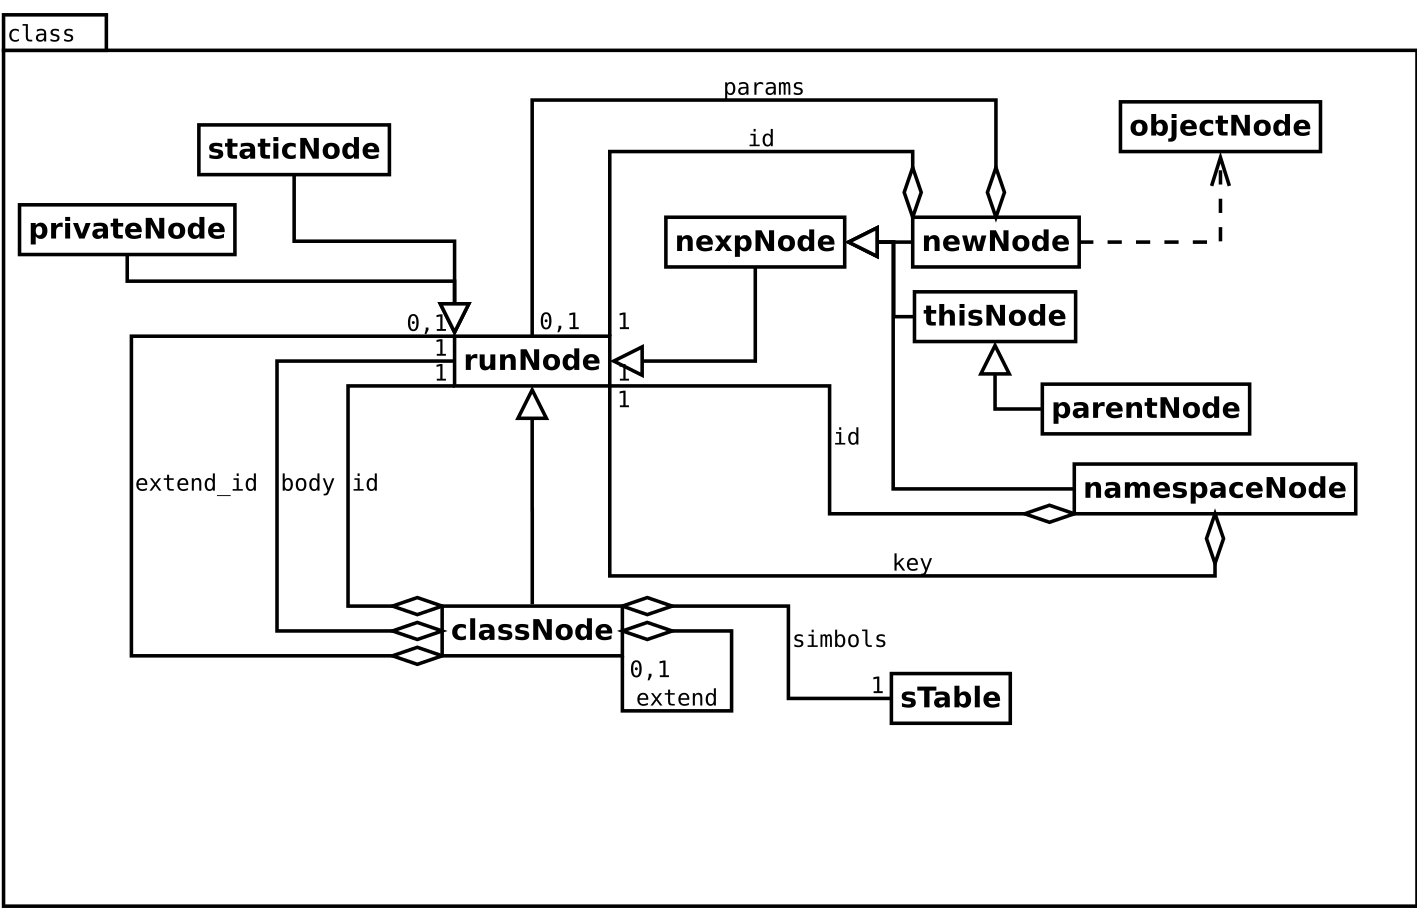
\includegraphics[scale=0.4]{class.png} \\
\end{center}

\paragraph {Objetos}
\begin{center}
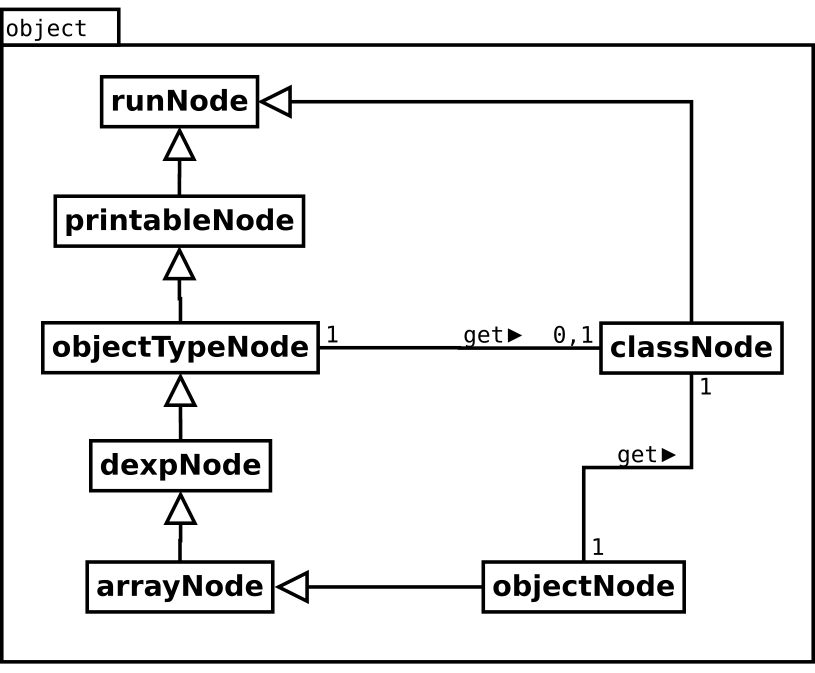
\includegraphics[scale=0.4]{object.png} \\
\end{center}

\paragraph {Listas}
\begin{center}
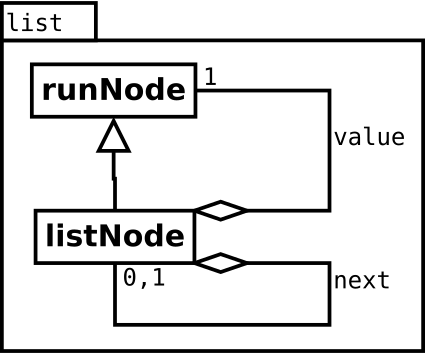
\includegraphics[scale=0.4]{list.png} \\
\end{center}

\paragraph {Pares clave/valor}
\begin{center}
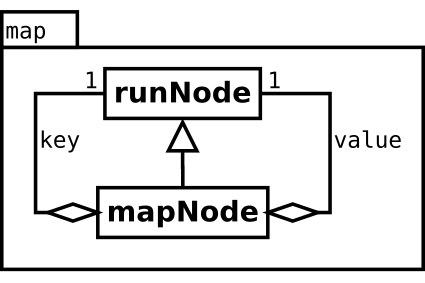
\includegraphics[scale=0.4]{map.png} \\
\end{center}

\paragraph {Etiquetas}
\begin{center}
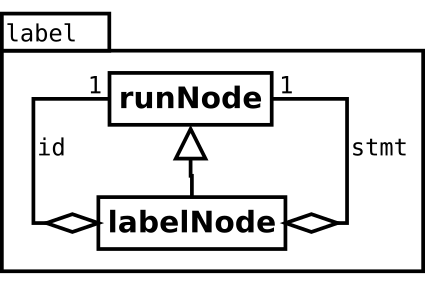
\includegraphics[scale=0.4]{label.png} \\
\end{center}

\paragraph {Definiciones globales}
\begin{center}
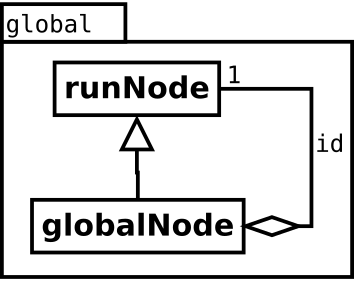
\includegraphics[scale=0.4]{global.png} \\
\end{center}

\paragraph {Generadores}
\begin{center}
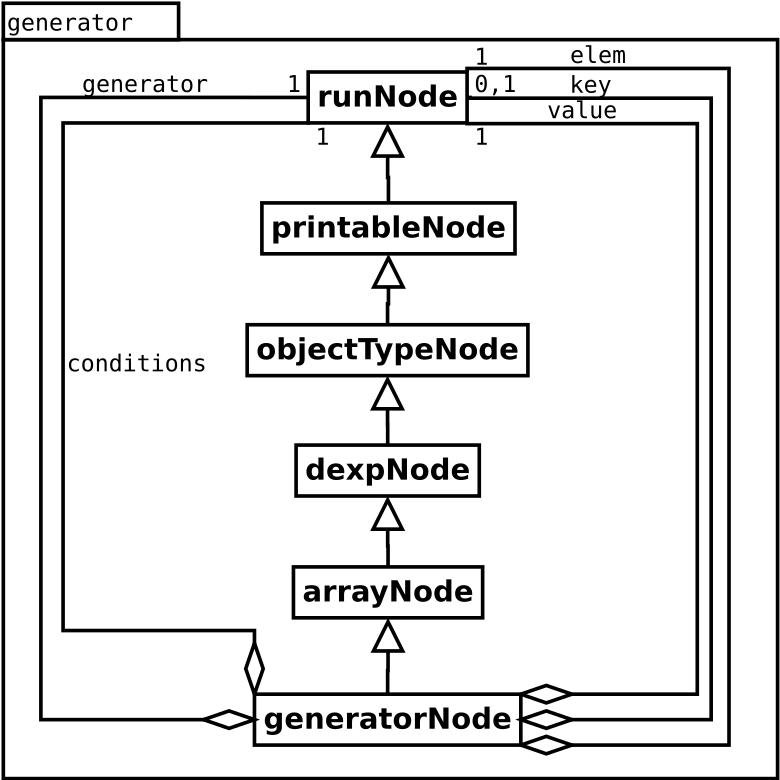
\includegraphics[scale=0.4]{generator.png} \\
\end{center}
% ----------------------------------------------------------------------
\pagebreak
\subsubsection {Asignaciones}
\begin{center}
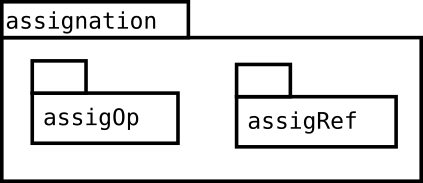
\includegraphics[scale=0.4]{assig-package.png} \\
\end{center}

\paragraph {Asignación}
\begin{center}
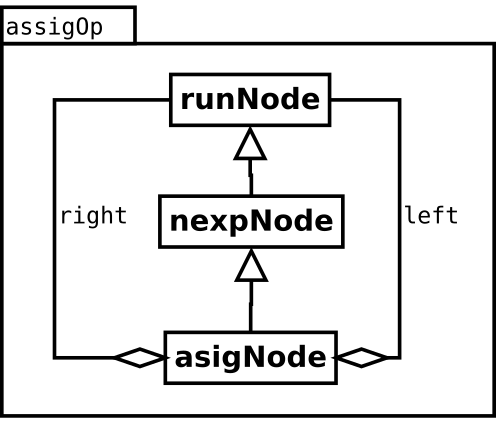
\includegraphics[scale=0.4]{assigNode.png} \\
\end{center}

\paragraph {Asignación de referencia}
\begin{center}
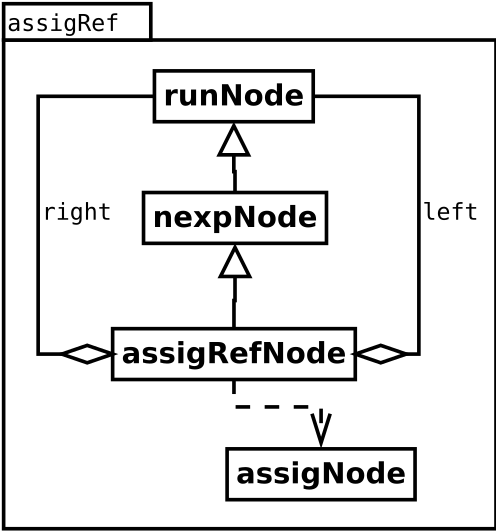
\includegraphics[scale=0.4]{assigRef.png} \\
\end{center}

% ----------------------------------------------------------------------
\pagebreak
\subsubsection {Operadores aritméticos}
\begin{center}
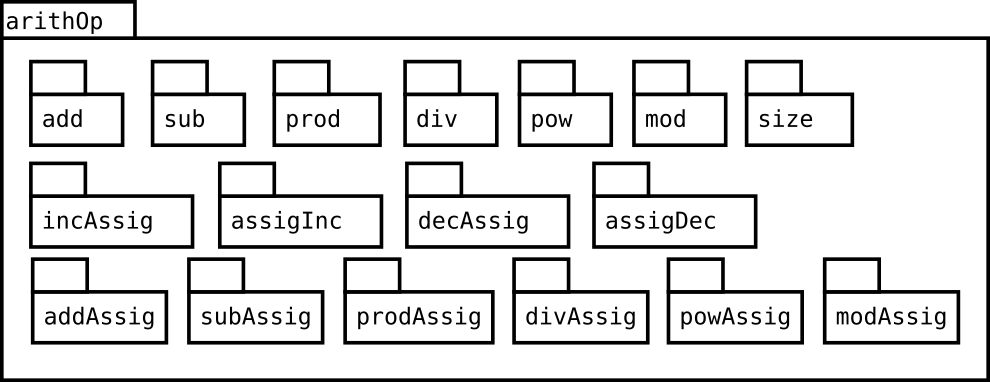
\includegraphics[scale=0.4]{arithOp-package.png} \\
\end{center}

\paragraph {Suma}
\begin{center}
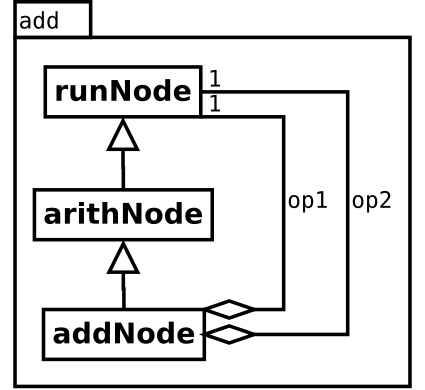
\includegraphics[scale=0.4]{add.png} \\
\end{center}

\paragraph {Diferencia}
\begin{center}
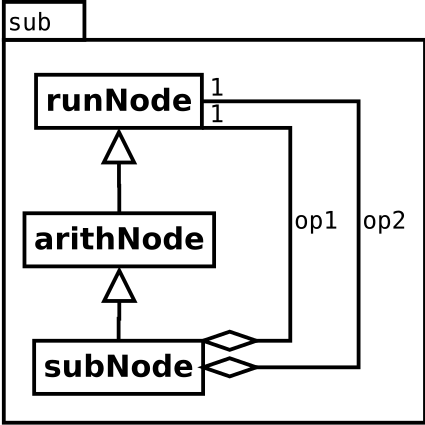
\includegraphics[scale=0.4]{sub.png} \\
\end{center}

\paragraph {Producto}
\begin{center}
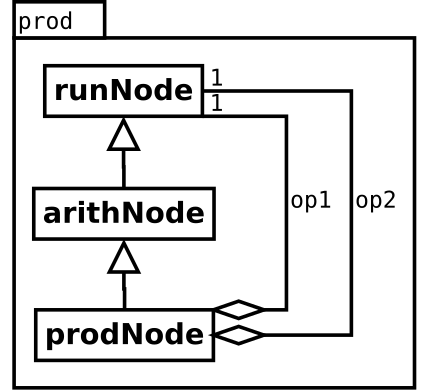
\includegraphics[scale=0.4]{prod.png} \\
\end{center}

\paragraph {División}
\begin{center}
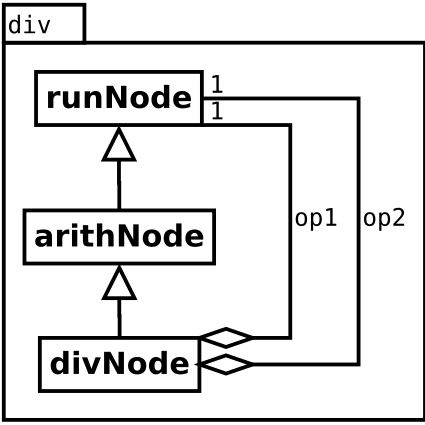
\includegraphics[scale=0.4]{div.png} \\
\end{center}

\paragraph {Potencia}
\begin{center}
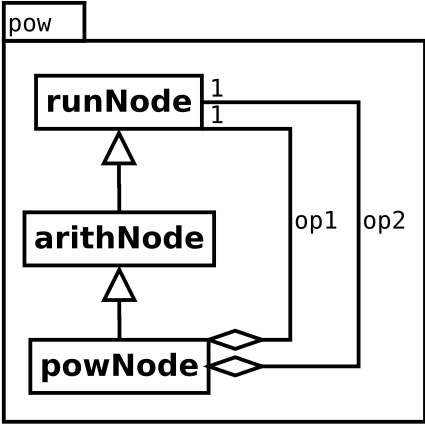
\includegraphics[scale=0.4]{pow.png} \\
\end{center}

\paragraph {Módulo}
\begin{center}
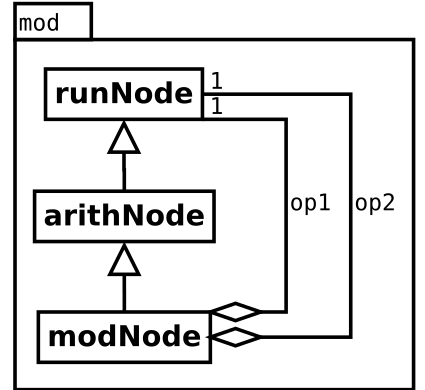
\includegraphics[scale=0.4]{mod.png} \\
\end{center}

\paragraph {Tamaño}
\begin{center}
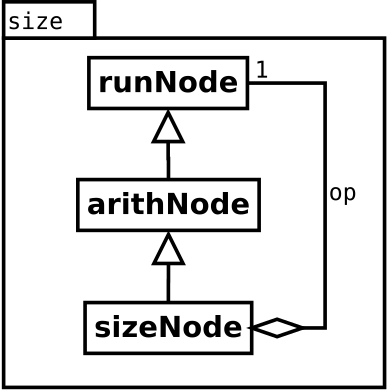
\includegraphics[scale=0.4]{size.png} \\
\end{center}

\paragraph {Incremento y asignación}
\begin{center}
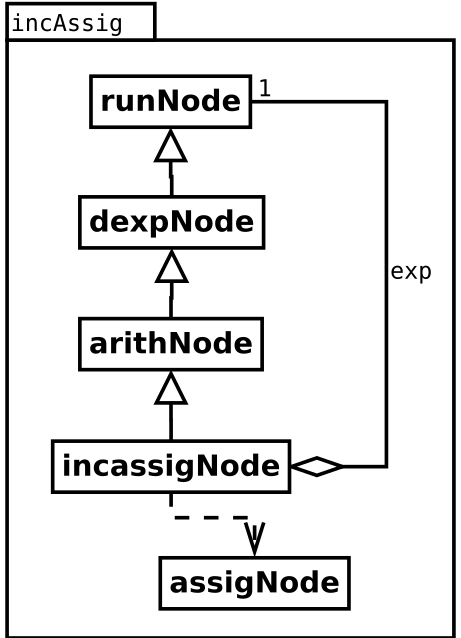
\includegraphics[scale=0.4]{incAssig.png} \\
\end{center}

\paragraph {Asignación e incremento}
\begin{center}
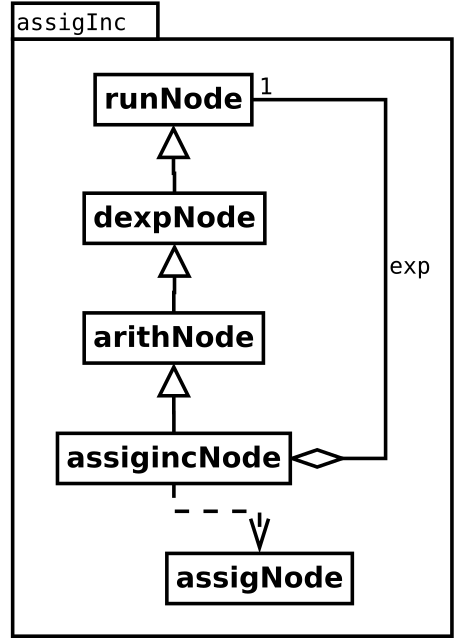
\includegraphics[scale=0.4]{assigInc.png} \\
\end{center}

\paragraph {Decremento y asignación}
\begin{center}
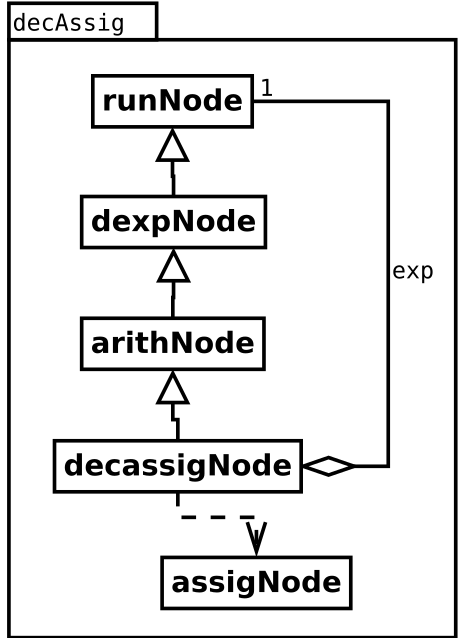
\includegraphics[scale=0.4]{decAssig.png} \\
\end{center}

\paragraph {Asignación y decremento}
\begin{center}
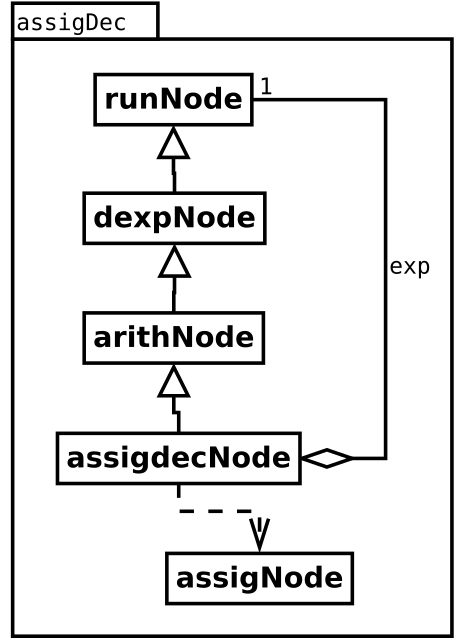
\includegraphics[scale=0.4]{assigDec.png} \\
\end{center}
% ----------------------------------------------------------------------
\pagebreak
\subsubsection {Operadores lógicos}
\begin{center}
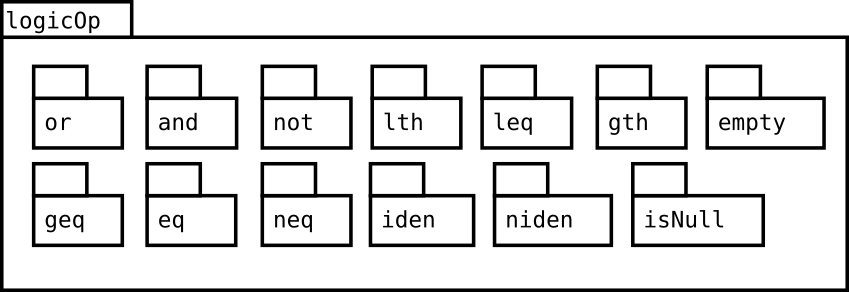
\includegraphics[scale=0.4]{logicOp-package.png} \\
\end{center}

\paragraph {Or}
\begin{center}
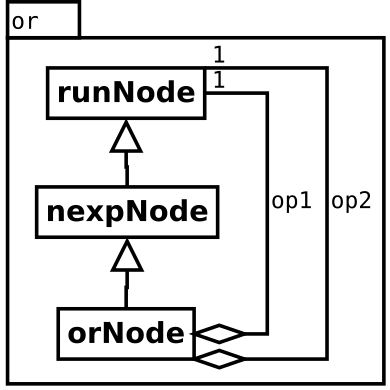
\includegraphics[scale=0.4]{or.png} \\
\end{center}

\paragraph {And}
\begin{center}
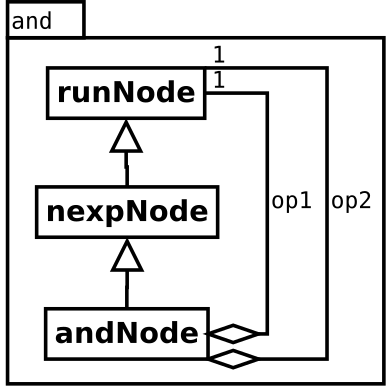
\includegraphics[scale=0.4]{and.png} \\
\end{center}

\paragraph {Negación}
\begin{center}
\includegraphics[scale=0.4]{not.png} \\
\end{center}


\paragraph {Igual que}
\begin{center}
\includegraphics[scale=0.4]{eq.png} \\
\end{center}

\paragraph {Distinto que}
\begin{center}
\includegraphics[scale=0.4]{neq.png} \\
\end{center}

\paragraph {Menor que}
\begin{center}
\includegraphics[scale=0.4]{lth.png} \\
\end{center}

\paragraph {Menor o igual que}
\begin{center}
\includegraphics[scale=0.4]{leq.png} \\
\end{center}

\paragraph {Mayor que}
\begin{center}
\includegraphics[scale=0.4]{gth.png} \\
\end{center}

\paragraph {Mayor o igual que}
\begin{center}
\includegraphics[scale=0.4]{geq.png} \\
\end{center}


\paragraph {Idéntico a}
\begin{center}
\includegraphics[scale=0.4]{iden.png} \\
\end{center}

\paragraph {No idéntico a}
\begin{center}
\includegraphics[scale=0.4]{niden.png} \\
\end{center}

\paragraph {Es nulo}
\begin{center}
\includegraphics[scale=0.4]{isNull.png} \\
\end{center}

\paragraph {Vacío}
\begin{center}
\includegraphics[scale=0.4]{empty.png} \\
\end{center}

% ----------------------------------------------------------------------

\pagebreak
\subsubsection {Operadores sobre cadenas}
\begin{center}
\includegraphics[scale=0.4]{stringOp-package.png} \\
\end{center}

\paragraph {Concatenación}
\begin{center}
\includegraphics[scale=0.4]{cat.png} \\
\end{center}

\paragraph {explode}
\begin{center}
\includegraphics[scale=0.4]{explode.png} \\
\end{center}

\paragraph {implode}
\begin{center}
\includegraphics[scale=0.4]{implode.png} \\
\end{center}

\paragraph {sprintf}
\begin{center}
\includegraphics[scale=0.4]{sprintf.png} \\
\end{center}

\paragraph {Buscar subcadena}
\begin{center}
\includegraphics[scale=0.4]{find.png} \\
\end{center}

\paragraph {Buscar y remplazar}
\begin{center}
\includegraphics[scale=0.4]{replace.png} \\
\end{center}

\paragraph {Remplazar subcadena}
\begin{center}
\includegraphics[scale=0.4]{subreplace.png} \\
\end{center}

\paragraph {Convertir a mayúsculas}
\begin{center}
\includegraphics[scale=0.4]{upper.png} \\
\end{center}

\paragraph {Convertir a minúsculas}
\begin{center}
\includegraphics[scale=0.4]{lower.png} \\
\end{center}

%~ \paragraph {Concatenación y asignación}
%~ Diagrama aún por realizar.
%~ \begin{center}
%~ \includegraphics[scale=0.4]{lower.png} \\
%~ \end{center}
% ----------------------------------------------------------------------
\pagebreak
\subsubsection {Operadores sobre array}
\begin{center}
\includegraphics[scale=0.4]{arrayOp-package.png} \\
\end{center}

\paragraph {Dividir en fragmentos}
\begin{center}
\includegraphics[scale=0.4]{chunk.png} \\
\end{center}

\paragraph {Reducir mediante función}
\begin{center}
\includegraphics[scale=0.4]{reduce.png} \\
\end{center}

\paragraph {Obtener último}
\begin{center}
\includegraphics[scale=0.4]{last.png} \\
\end{center}

\paragraph {Obtener primero}
\begin{center}
\includegraphics[scale=0.4]{first.png} \\
\end{center}

\paragraph {Insertar en posición}
\begin{center}
\includegraphics[scale=0.4]{insert.png} \\
\end{center}

\paragraph {Eliminar posición}
\begin{center}
\includegraphics[scale=0.4]{delete.png} \\
\end{center}

\paragraph {Insertar al inicio}
\begin{center}
\includegraphics[scale=0.4]{unshift.png} \\
\end{center}

\paragraph {Insertar al final}
\begin{center}
\includegraphics[scale=0.4]{push.png} \\
\end{center}

\paragraph {Eliminar del inicio}
\begin{center}
\includegraphics[scale=0.4]{shift.png} \\
\end{center}

\paragraph {Eliminar del final}
\begin{center}
\includegraphics[scale=0.4]{pop.png} \\
\end{center}



% ----------------------------------------------------------------------

\pagebreak
\subsubsection {Operadores sobre expresiones regulares}
\begin{center}
\includegraphics[scale=0.4]{regexpOp-package.png} \\
\end{center}

\paragraph {Crear expresión regular}
\begin{center}
\includegraphics[scale=0.4]{newRegExp.png} \\
\end{center}

\paragraph {match}
\begin{center}
\includegraphics[scale=0.4]{match.png} \\
\end{center}

\paragraph {search}
\begin{center}
\includegraphics[scale=0.4]{search.png} \\
\end{center}

% ----------------------------------------------------------------------
\pagebreak
\subsubsection {Conversión de tipos}
\begin{center}
\includegraphics[scale=0.4]{convOp-package.png} \\
\end{center}

\paragraph {Conversión a lógico}
\begin{center}
\includegraphics[scale=0.4]{boolconv.png} \\
\end{center}

\paragraph {Conversión a entero}
\begin{center}
\includegraphics[scale=0.4]{intconv.png} \\
\end{center}

\paragraph {Conversión a flotante}
\begin{center}
\includegraphics[scale=0.4]{floatconv.png} \\
\end{center}

\paragraph {Conversión a cadena}
\begin{center}
\includegraphics[scale=0.4]{strconv.png} \\
\end{center}
% ----------------------------------------------------------------------

\pagebreak
\subsubsection {Operadores de acceso}
\begin{center}
\includegraphics[scale=0.4]{accessOp-package.png} \\
\end{center}

\paragraph {Acceso a clave} 
\begin{center}
\includegraphics[scale=0.4]{get.png} \\
\end{center}

\paragraph {Acceso a función} 
\begin{center}
\includegraphics[scale=0.4]{getFunc.png} \\
\end{center}

\paragraph {Acceso a variable de entorno} 
\begin{center}
\includegraphics[scale=0.4]{getEnvSys.png} \\
\end{center}
% ----------------------------------------------------------------------

\pagebreak
\subsubsection {Operadores condicionales} 
\begin{center}
\includegraphics[scale=0.4]{condOp-package.png} \\
\end{center}

\paragraph {Ternario} 
\begin{center}
\includegraphics[scale=0.4]{tern.png} \\
\end{center}

\paragraph {Fusión de nulos} 
\begin{center}
\includegraphics[scale=0.4]{nullCoalescing.png} \\
\end{center}
% ----------------------------------------------------------------------

\pagebreak
\subsubsection {Operadores de entrada/salida} 
\begin{center}
\includegraphics[scale=0.4]{ioOp-package.png} \\
\end{center}
\paragraph {Salida estándar} 
\begin{center}
\includegraphics[scale=0.4]{output.png} \\
\end{center}
\paragraph {Entrada estándar} 
\begin{center}
\includegraphics[scale=0.4]{input.png} \\
\end{center}
% ----------------------------------------------------------------------
\pagebreak
\subsubsection {Operadores informativos} 
\begin{center}
\includegraphics[scale=0.4]{infoOp-package.png} \\
\end{center}

\paragraph {Tipo de} 
\begin{center}
\includegraphics[scale=0.4]{typeOf.png} \\
\end{center}

\paragraph {Tamaño de} 
\begin{center}
\includegraphics[scale=0.4]{sizeOf.png} \\
\end{center}

\paragraph {Información sobre} 
\begin{center}
\includegraphics[scale=0.4]{datInfo.png} \\
\end{center}
% ----------------------------------------------------------------------

\pagebreak
\subsubsection {Procesos} 
\begin{center}
\includegraphics[scale=0.4]{processOp-package.png} \\
\end{center}

\begin{multicols}{2}
   \paragraph {Crear proceso} 
   \begin{center}
   \includegraphics[scale=0.4]{fork.png} \\
   \end{center}
\columnbreak
   \paragraph {Esperar finalización} 
   \begin{center}
   \includegraphics[scale=0.4]{wait.png} \\
   \end{center}
\end{multicols}


\begin{multicols}{2}
   \paragraph {Obtener identificador } 
   \begin{center}
   \includegraphics[scale=0.4]{getpid.png} \\
   \end{center}
\columnbreak
   \paragraph {Obtener identificador padre} 
   \begin{center}
   \includegraphics[scale=0.4]{getppid.png} \\
   \end{center}
\end{multicols}


\begin{multicols}{2}
   \paragraph {Ejecutar como proceso} 
   \begin{center}
   \includegraphics[scale=0.4]{process.png} \\
   \end{center}
\columnbreak
   \paragraph {Salir de proceso} 
   \begin{center}
   \includegraphics[scale=0.4]{exitProcess.png} \\
   \end{center}
\end{multicols}


\begin{multicols}{2}
   \paragraph {Señal a proceso} 
   \begin{center}
   \includegraphics[scale=0.4]{signal.png} \\
   \end{center}
\columnbreak
   \paragraph {Manejador de señales} 
   \begin{center}
   \includegraphics[scale=0.4]{signalhandler.png} \\
   \end{center}
\end{multicols}


\begin{multicols}{2}
   \paragraph {Evaluar cadena} 
   \begin{center}
   \includegraphics[scale=0.4]{eval.png} \\
   \end{center}
\columnbreak
   \paragraph {Ejecutar comando del sistema} 
   \begin{center}
   \includegraphics[scale=0.4]{exec.png} \\
   \end{center}
\end{multicols}
% ----------------------------------------------------------------------

\pagebreak
\subsubsection {Ficheros} 
\begin{center}
\includegraphics[scale=0.4]{fileOp-package.png} \\
\end{center}

\begin{multicols}{2}
   \paragraph {Obtener un flujo a fichero} 
   \begin{center}
   \includegraphics[scale=0.4]{file.png} \\
   \end{center}

   \paragraph {Escribir en flujo a fichero} 
   \begin{center}
   \includegraphics[scale=0.4]{fput.png} \\
   \end{center}

   \paragraph {Leer de flujo a fichero} 
   \begin{center}
   \includegraphics[scale=0.4]{fget.png} \\
   \end{center}

   \paragraph {Cambiar posición en fichero} 
   \begin{center}
   \includegraphics[scale=0.4]{fseek.png} \\
   \end{center}
\columnbreak
\paragraph {Obtener posición en flujo a fichero} 
   \begin{center}
   \includegraphics[scale=0.4]{ftell.png} \\
   \end{center}

   \paragraph {Cerrar flujo a fichero} 
   \begin{center}
   \includegraphics[scale=0.4]{fclose.png} \\
   \end{center}

   \paragraph {Leer fichero} 
   \begin{center}
   \includegraphics[scale=0.4]{fread.png} \\
   \end{center}

   \paragraph {Escribir en fichero} 
   \begin{center}
   \includegraphics[scale=0.4]{fwrite.png} \\
   \end{center}
\end{multicols}

\paragraph {Escribir al final de fichero} 
\begin{center}
\includegraphics[scale=0.4]{fappend.png} \\
\end{center}
% ----------------------------------------------------------------------
 
\begin{multicols}{2}
\subsubsection {Fechas}
   \begin{center}
   \includegraphics[scale=0.4]{dateOp-package.png} \\
   \end{center}
   \paragraph {Tiempo Unix} 
   \begin{center}
   \includegraphics[scale=0.4]{time.png} \\
   \end{center}
\columnbreak
   \paragraph {Fecha y hora con formato} 
   \begin{center}
   \includegraphics[scale=0.4]{date.png} \\
   \end{center}

   \paragraph {sleep} 
   \begin{center}
   \includegraphics[scale=0.4]{sleep.png} \\
   \end{center}
\end{multicols}
% ----------------------------------------------------------------------

\subsubsection {Errores} 
%~ \begin{center}
%~ \includegraphics[scale=0.4]{error-package.png} \\
%~ \end{center}
%~ 
%~ \paragraph {Error} 
\begin{center}
\includegraphics[scale=0.4]{errorException.png} \\
\end{center}

%~ \paragraph {Manejador de errores } 
%~ Diagrama aún por realizar
%~ \begin{center}
%~ \includegraphics[scale=0.4]{errorhandler.png} \\
%~ \end{center}

%~ \paragraph {Manejador de excepciones no capturadas} 
%~ Diagrama aún por realizar
%~ \begin{center}
%~ \includegraphics[scale=0.4]{errorhandler.png} \\
%~ \end{center}
% ----------------------------------------------------------------------

\pagebreak
\subsubsection {Extensiones} 
\begin{center}
\includegraphics[scale=0.4]{extensions-package.png} \\
\end{center}

\begin{center}
\includegraphics[scale=0.4]{plugins.png} \\
\end{center}

\paragraph{Biblioteca GNU de internacionalización (gettext)}
\begin{center}
\includegraphics[scale=0.4]{gettext-ext-package.png} \\
\end{center}
\subparagraph {gettext}
\begin{center}
\includegraphics[scale=0.4]{gettext.png} \\
\end{center}
\begin{multicols}{2}
\subparagraph {setlocale}
\begin{center}
\includegraphics[scale=0.4]{setlocale.png} \\
\end{center}
\subparagraph {dgettext}
\begin{center}
\includegraphics[scale=0.4]{dgettext.png} \\
\end{center}
\columnbreak
\subparagraph {bindtextdomain}
\begin{center}
\includegraphics[scale=0.4]{bindtextdomain.png} \\
\end{center}
\subparagraph {textdomain}
\begin{center}
\includegraphics[scale=0.4]{textdomain.png} \\
\end{center}
\end{multicols}

\subsubsection {rTree} 
El intérprete OMI tiene la capacidad de generar una salida relativa
a su estado y funcionamiento. Para completar el proyecto se precisa 
de una herramienta capaz de interpretar y representar este estado 
interno de forma gráfica y textual. 

El modelo de datos del cliente OMI se define de forma similar al intérprete.
La principal diferencia es que en el intérprete este modelo de datos se usa para procesar y 
ejecutar el código fuente, mientras que en el cliente se usa para representar gráficamente 
el proceso llevado a cabo. Es por ello que el modelo de datos del cliente es más abstracto. 

\begin{center}
\includegraphics[scale=0.6]{rtree.png} \\
\end{center}

%~ \paragraph {Operaciones sobre un SGBD Mysql}
%~ \begin{center}
%~ \includegraphics[scale=0.4]{mysql-ext-package.png} \\
%~ \end{center}
%~ \subparagraph {Abrir conexión}
%~ \begin{center}
%~ \includegraphics[scale=0.4]{db.png} \\
%~ \end{center}
%~ 
%~ \subparagraph {Consulta}
%~ \begin{center}
%~ \includegraphics[scale=0.4]{dbQuery.png} \\
%~ \end{center}
%~ 
%~ \subparagraph {Cerrar conexión}
%~ Diagrama aún por realizar.
%~ \begin{center}
%~ \includegraphics[scale=0.4]{dbClose.png} \\
%~ \end{center}
%~ 
%~ \subparagraph {Insertar datos}
%~ \begin{center}
%~ \includegraphics[scale=0.4]{dbInsert.png} \\
%~ \end{center}
%~ 
%~ \subparagraph {Seleccionar datos}
%~ \begin{center}
%~ \includegraphics[scale=0.4]{dbSelect.png} \\
%~ \end{center}
%~ 
%~ \subparagraph {Actualizar datos}
%~ \begin{center}
%~ \includegraphics[scale=0.4]{dbUpdate.png} \\
%~ \end{center}
%~ 
%~ \subparagraph {Eliminar datos}
%~ \begin{center}
%~ \includegraphics[scale=0.4]{dbDelete.png} \\
%~ \end{center}
%~ 
%~ % ----------------------------------------------------------------------
